\documentclass{article}

% chinese fonts
\usepackage{ctex}

% math fonts
\usepackage{amsmath}
\usepackage{amsthm}
\usepackage{amssymb}
\usepackage{bm}

% figures
\usepackage{tikz}
\usepackage{graphicx}
\graphicspath{{./figures/}}

% tables
\usepackage{tabularx}
\usepackage{booktabs}
\usepackage{multirow}

% codes
\usepackage{listings}
\lstset{language     = Matlab,
        basicstyle   = \ttfamily,
        keywordstyle = \color{cyan},
        rulecolor    = \color{black},
        commentstyle = \color{green},
        keepspaces   = true,
        tabsize      = 4,
}

% hyperlinks
\usepackage{hyperref}
\hypersetup{
  breaklinks,
  colorlinks = true,
  citecolor  = blue,
  linkcolor  = red,
  urlcolor   = magenta,
}

% algorithms
\usepackage{algorithm}
\usepackage{algorithmic}

% bibliography
\usepackage[sort&compress,numbers]{natbib}

% About:  Macros for Vector, Matrix, Tensor, Math Operator and Misc
% Author: Jingxuan Yang

% vectors
\newcommand{\va}{\bm{a}}       \newcommand{\vah}{\hat{\bm{a}}}        \newcommand{\ah}{\hat{a}}    \newcommand{\vat}{\tilde{\bm{a}}}       \newcommand{\at}{\tilde{a}}
\newcommand{\vb}{\bm{b}}       \newcommand{\vbh}{\hat{\bm{b}}}        \newcommand{\bh}{\hat{b}}    \newcommand{\vbt}{\tilde{\bm{b}}}       \newcommand{\bt}{\tilde{b}}
\newcommand{\vc}{\bm{c}}       \newcommand{\vch}{\hat{\bm{c}}}        \newcommand{\ch}{\hat{c}}    \newcommand{\vct}{\tilde{\bm{c}}}       \newcommand{\ct}{\tilde{c}}
\newcommand{\vd}{\bm{d}}       \newcommand{\vdh}{\hat{\bm{d}}}        \newcommand{\dhat}{\hat{d}}  \newcommand{\vdt}{\tilde{\bm{d}}}       \newcommand{\dt}{\tilde{d}}
\newcommand{\ve}{\bm{e}}       \newcommand{\veh}{\hat{\bm{e}}}        \newcommand{\eh}{\hat{e}}    \newcommand{\vet}{\tilde{\bm{e}}}       \newcommand{\et}{\tilde{e}}
\newcommand{\vf}{\bm{f}}       \newcommand{\vfh}{\hat{\bm{f}}}        \newcommand{\fh}{\hat{f}}    \newcommand{\vft}{\tilde{\bm{f}}}       \newcommand{\ft}{\tilde{f}}
\newcommand{\vg}{\bm{g}}       \newcommand{\vgh}{\hat{\bm{g}}}        \newcommand{\gh}{\hat{g}}    \newcommand{\vgt}{\tilde{\bm{g}}}       \newcommand{\gt}{\tilde{g}}
\newcommand{\vh}{\bm{h}}     \newcommand{\vhh}{\hat{\bm{h}}}        \newcommand{\hh}{\hat{h}}    \newcommand{\vht}{\tilde{\bm{h}}}       \newcommand{\htild}{\tilde{h}}
\newcommand{\vi}{\bm{i}}       \newcommand{\vih}{\hat{\bm{i}}}        \newcommand{\ih}{\hat{i}}    \newcommand{\vit}{\tilde{\bm{i}}}       \newcommand{\itild}{\tilde{i}}
\newcommand{\vj}{\bm{j}}       \newcommand{\vjh}{\hat{\bm{j}}}        \newcommand{\jh}{\hat{j}}    \newcommand{\vjt}{\tilde{\bm{j}}}       \newcommand{\jt}{\tilde{j}}
\newcommand{\vk}{\bm{k}}       \newcommand{\vkh}{\hat{\bm{k}}}        \newcommand{\kh}{\hat{k}}    \newcommand{\vkt}{\tilde{\bm{k}}}       \newcommand{\kt}{\tilde{k}}
\newcommand{\vl}{\bm{l}}       \newcommand{\vlh}{\hat{\bm{l}}}        \newcommand{\lh}{\hat{l}}    \newcommand{\vlt}{\tilde{\bm{l}}}       \newcommand{\lt}{\tilde{l}}
\newcommand{\vm}{\bm{m}}       \newcommand{\vmh}{\hat{\bm{m}}}        \newcommand{\mh}{\hat{m}}    \newcommand{\vmt}{\tilde{\bm{m}}}       \newcommand{\mt}{\tilde{m}}
\newcommand{\vn}{\bm{n}}       \newcommand{\vnh}{\hat{\bm{n}}}        \newcommand{\nh}{\hat{n}}    \newcommand{\vnt}{\tilde{\bm{n}}}       \newcommand{\nt}{\tilde{n}}
\newcommand{\vo}{\bm{o}}       \newcommand{\voh}{\hat{\bm{o}}}        \newcommand{\oh}{\hat{o}}    \newcommand{\vot}{\tilde{\bm{o}}}       \newcommand{\ot}{\tilde{o}}
\newcommand{\vp}{\bm{p}}       \newcommand{\vph}{\hat{\bm{p}}}        \newcommand{\ph}{\hat{p}}    \newcommand{\vpt}{\tilde{\bm{p}}}       \newcommand{\pt}{\tilde{p}}
\newcommand{\vq}{\bm{q}}       \newcommand{\vqh}{\hat{\bm{q}}}        \newcommand{\qh}{\hat{q}}    \newcommand{\vqt}{\tilde{\bm{q}}}       \newcommand{\qt}{\tilde{q}}
\newcommand{\vr}{\bm{r}}       \newcommand{\vrh}{\hat{\bm{r}}}        \newcommand{\rh}{\hat{r}}    \newcommand{\vrt}{\tilde{\bm{r}}}       \newcommand{\rt}{\tilde{r}}
\newcommand{\vs}{\bm{s}}       \newcommand{\vsh}{\hat{\bm{s}}}        \newcommand{\sh}{\hat{s}}    \newcommand{\vst}{\tilde{\bm{s}}}       \newcommand{\st}{\tilde{s}}
\newcommand{\vt}{\bm{t}}       \newcommand{\vth}{\hat{\bm{t}}}        \newcommand{\that}{\hat{t}}  \newcommand{\vtt}{\tilde{\bm{t}}}       \newcommand{\ttil}{\tilde{t}}
\newcommand{\vu}{\bm{u}}       \newcommand{\vuh}{\hat{\bm{u}}}        \newcommand{\uh}{\hat{u}}    \newcommand{\vut}{\tilde{\bm{u}}}       \newcommand{\ut}{\tilde{u}}
\newcommand{\vv}{\bm{v}}       \newcommand{\vvh}{\hat{\bm{v}}}        \newcommand{\vhat}{\hat{v}}    \newcommand{\vvt}{\tilde{\bm{v}}}       \newcommand{\vtild}{\tilde{v}}
\newcommand{\vw}{\bm{w}}       \newcommand{\vwh}{\hat{\bm{w}}}        \newcommand{\wh}{\hat{w}}    \newcommand{\vwt}{\tilde{\bm{w}}}       \newcommand{\wt}{\tilde{w}}
\newcommand{\vx}{\bm{x}}       \newcommand{\vxh}{\hat{\bm{x}}}        \newcommand{\xh}{\hat{x}}    \newcommand{\vxt}{\tilde{\bm{x}}}       \newcommand{\xt}{\tilde{x}}
\newcommand{\vy}{\bm{y}}       \newcommand{\vyh}{\hat{\bm{y}}}        \newcommand{\yh}{\hat{y}}    \newcommand{\vyt}{\tilde{\bm{y}}}       \newcommand{\yt}{\tilde{y}}
\newcommand{\vz}{\bm{z}}       \newcommand{\vzh}{\hat{\bm{z}}}        \newcommand{\zh}{\hat{z}}    \newcommand{\vzt}{\tilde{\bm{z}}}       \newcommand{\zt}{\tilde{z}}

\newcommand{\valpha}{\bm{\alpha}}
\newcommand{\vbeta}{\bm{\beta}}
\newcommand{\vgamma}{\bm{\gamma}}
\newcommand{\vtheta}{\bm{\theta}}
\newcommand{\vlambda}{\bm{\lambda}}
\newcommand{\vmu}{\bm{\mu}}
\newcommand{\vomega}{\bm{\omega}}

\newcommand{\mSigma}{\bm{\Sigma}}

\newcommand{\Fc}{\mathcal{F}}
\newcommand{\Xc}{\mathcal{X}}
\newcommand{\Yc}{\mathcal{Y}}
\newcommand{\Zc}{\mathcal{Z}}
\newcommand{\Gc}{\mathcal{G}}
\newcommand{\Hc}{\mathcal{H}}
\newcommand{\Dc}{\mathcal{D}}
\newcommand{\Cc}{\mathcal{C}}
\newcommand{\Rc}{\mathcal{R}}

% matrices
\newcommand{\ma}{\bm{A}}
\newcommand{\mb}{\bm{B}}
\newcommand{\md}{\bm{D}}
\newcommand{\mH}{\bm{H}}
\newcommand{\mE}{\bm{E}}
\newcommand{\mi}{\bm{I}}
\newcommand{\mk}{\bm{K}}
\newcommand{\ml}{\bm{L}}
\newcommand{\mn}{\bm{N}}
\newcommand{\mP}{\bm{P}}
\newcommand{\mq}{\bm{Q}}
\newcommand{\mr}{\bm{R}}
\newcommand{\mU}{\bm{u}}
\newcommand{\mv}{\bm{v}}
\newcommand{\mw}{\bm{W}}
\newcommand{\mx}{\bm{X}}
\newcommand{\my}{\bm{Y}}
\newcommand{\mz}{\bm{Z}}

% tensors
\newcommand{\tp}{\mathsf{P}}
\newcommand{\tu}{\mathsf{U}}
\newcommand{\tx}{\mathsf{X}}
\newcommand{\ty}{\mathsf{Y}}
\newcommand{\tz}{\mathsf{Z}}
\newcommand{\tw}{\mathsf{W}}
\newcommand{\tf}{\mathsf{F}}
\newcommand{\ta}{\mathsf{A}}
\renewcommand{\th}{\mathsf{H}}

% norms
\newcommand{\mynorm}[2]{\| {#1} \|_{#2}}
\newcommand{\norm}[2]{\mynorm{#1}{#2}}
\newcommand{\bignorm}[2]{\left\| {#1} \right\|_{#2}}
\newcommand{\norml}[1]{\mynorm{#1}{1}}
\newcommand{\bignorml}[1]{\bignorm{#1}{1}}
\newcommand{\infnorm}[1]{\mynorm{#1}{\infty}}
\newcommand{\biginfnorm}[1]{\bignorm{#1}{\infty}}
\newcommand{\oneinf}{\ell_{1,\infty}}
\newcommand{\onetwo}{\ell_{1,2}}
\newcommand{\oneinfnorm}[1]{\mynorm{#1}{1,\infty}}
\newcommand{\bigoneinf}[1]{\bignorm{#1}{1,\infty}}
\newcommand{\onetwonorm}[1]{\mynorm{#1}{1,2}}
\newcommand{\bigonetwo}[1]{\bignorm{#1}{1,2}}
\newcommand{\enorm}[1]{\mynorm{#1}{2}}
\newcommand{\bigenorm}[1]{\bignorm{#1}{2}}
\newcommand{\znorm}[1]{\mynorm{#1}{0}}
\newcommand{\bigznorm}[1]{\bignorm{#1}{0}}
\newcommand{\frob}[1]{\|{#1}\|_{\text{F}}}
\newcommand{\bigfrob}[1]{\bignorm{#1}{\text{F}}}
\newcommand{\grpnorm}[2]{\norm{#1}{\text{Gr}(#2)}}

% math operators
\DeclareMathOperator*{\argmin}{argmin}
\DeclareMathOperator*{\argmax}{argmax}
\DeclareMathOperator{\divg}{div}
\DeclareMathOperator{\dom}{dom}
\DeclareMathOperator{\interior}{int}
\DeclareMathOperator{\ri}{ri}
\DeclareMathOperator{\sgn}{sgn}
\DeclareMathOperator{\trace}{Tr}
\DeclareMathOperator{\diag}{diag}
\DeclareMathOperator{\rank}{rank}
\DeclareMathOperator{\range}{range}
\DeclareMathOperator{\vect}{vec}
\DeclareMathOperator{\prox}{prox}
\DeclareMathOperator{\intr}{int}
\DeclareMathOperator{\relint}{ri}

% misc
\newcommand{\gs}{\geqslant}
\newcommand{\ls}{\leqslant}
\newcommand{\set}[1]{\left\{ {#1}\right\}}

\newcommand{\defeq}{\ \stackrel{\text{def}}{=}\ }
\newcommand{\ip}[2]{\left\langle#1, #2\right\rangle}
\newcommand{\reals}{\mathbb{R}}
\newcommand{\complex}{\mathbb{C}}
\newcommand{\half}{\frac{1}{2}}

\newtheorem{theorem}{Theorem}
\newtheorem{lemma}[theorem]{Lemma}
\newtheorem{proposition}[theorem]{Proposition}
\newtheorem{remark}[theorem]{Remark}
\newtheorem{corollary}[theorem]{Corollary}
\newtheorem{definition}[theorem]{Definition}


\setlength{\oddsidemargin}{-0.25 in}
\setlength{\evensidemargin}{-0.25 in} 
\setlength{\topmargin}{-0.25in} 
\setlength{\textwidth}{7 in} 
\setlength{\textheight}{8.5 in}
\setlength{\headsep}{0.25 in} 
\setlength{\parindent}{0 in}
\setlength{\parskip}{0.1 in}

\newcommand{\homework}[5]{
  \pagestyle{myheadings} 
  \thispagestyle{plain}
  \newpage
  \setcounter{page}{1} 
  \setcounter{section}{#5} 
  \noindent
  \begin{center}
    \framebox{ 
      \vbox{
        \vspace{2mm} 
        \hbox to 6.28in { {\bf
        THU-70250043-0,~Pattern~Recognition~(Spring 2021) \hfill Homework: 12} }
        \vspace{6mm} 
        \hbox to 6.28in { {\Large \hfill #1 \hfill} }
        \vspace{6mm} 
        \hbox to 6.28in { {\it Lecturer: #2 \hfill} }
        \vspace{2mm} 
        \hbox to 6.28in { {\it \hspace{14mm} #3 \hfill} }
        \vspace{2mm} 
        \hbox to 6.28in { {\it Student: #4 \hfill} }
        \vspace{2mm} 
      } 
    }
  \end{center}
  \markboth{#1}{#1} 
  \vspace*{4mm} 
}

\begin{document}

\homework{Ensemble}{Changshui Zhang \hspace{5mm} {\tt zcs@mail.tsinghua.edu.cn}}{Hong Zhao \hspace{16mm} {\tt vzhao@tsinghua.edu.cn}}{Jingxuan Yang \hspace{10mm} {\tt yangjx20@mails.tsinghua.edu.cn}}{8}


\section*{Bagging}\label{problem:1}

In practice, we have only a single data set, and \emph{bagging} is a method to introduce variability between different models within the committee based on one data set. A committee can be viewed as a set of individual models on which we average our predictions.

The very first step is to use \emph{bootstrap} data sets. After we have generated $M$ bootstrap data sets, we then use each to train a separate predictive model $y_{m}$ where $m = 1,2,\dots, M.$ Then the prediction is given by
\begin{equation}
  y_{\text{COM}}=\frac{1}{M}\sum_{m=1}^{M}y_{m}(\vx).
  \label{eq:y_com}
\end{equation}

Suppose the true regression function that we are trying to predict is given by $h(\vx)$, so that the output of each of the models can be written as the true value plus an error in the form
\begin{equation}
  y_{m}(\vx)=h(\vx)+\epsilon_{m}(\vx).
\end{equation}

The average sum-of-square error then takes the form
\begin{eqnarray}
\mathbb{E}_{\vx}[\{y_{m}(\vx)-h(\vx)\}^{2}]=\mathbb{E}_{\vx}[\epsilon_{m}^{2}(\vx)] ,
\end{eqnarray}
where $\mathbb{E}_{\vx}$ denotes expectation with respect to the distribution of the input vector $\vx$.

The average error made by the models acting individually is therefore
\begin{equation}
  E_{\text{AV}}=\frac{1}{M}\sum_{m=1}^{M}\mathbb{E}_{\vx}[\epsilon_{m}^{2}(\vx)].
\end{equation}

Similarly, the expected error from equation (\ref{eq:y_com}) is given by
\begin{equation}
  \begin{aligned}
    E_{\text{COM}}
    &=\mathbb{E}_{\vx}\left[\left\{\frac{1}{M}\sum_{m=1}^{M}y_{m}(\vx)-h(\vx)\right\}^{2}\right] \\
    &=\mathbb{E}_{\vx}\left[\left\{\frac{1}{M}\sum_{m=1}^{M}\epsilon_{m}(\vx)\right\}^{2}\right]. \\
  \end{aligned}
\end{equation}

1.1 Assume that errors have zero mean and are uncorrelated
\begin{equation}
  \begin{aligned}
    \mathbb{E}_{\vx}[\epsilon_{m}(\vx)]&=0, \\
    \mathbb{E}_{\vx}[\epsilon_{m}(\vx)\epsilon_{l}(\vx)]&=0,~\forall~m\neq l.
  \end{aligned}
\end{equation}

Please prove that
\begin{equation}
  E_{\text{COM}}=\frac{1}{M}E_{\text{AV}}.
\end{equation}

解: 由误差不相关可得
\begin{equation}
  \begin{aligned}
    E_{\text{COM}}
    &=\mathbb{E}_{\vx}\left[\left\{\frac{1}{M}\sum_{m=1}^{M}\epsilon_{m}(\vx)\right\}^{2}\right]\\
    &=\frac{1}{M^2}\mathbb{E}_{\vx}\left[\left\{\sum_{m=1}^{M}\epsilon_{m}(\vx)\right\}^{2}\right]\\
    &=\frac{1}{M^2}\mathbb{E}_{\vx}\left[\sum_{m=1}^{M}\sum_{l=1}^{M}\epsilon_{m}(\vx)\epsilon_{l}(\vx)\right]\\
    &=\frac{1}{M^2}\mathbb{E}_{\vx}\left[\sum_{m=1}^{M}\epsilon_{m}^2(\vx)\right]\\
    &=\frac{1}{M^2}\sum_{m=1}^{M}\mathbb{E}_{\vx}[\epsilon_{m}^2(\vx)]\\
    &=\frac{1}{M}E_{\text{AV}}\\
  \end{aligned}
\end{equation}

1.2 In practice, the errors are typically highly correlated. Show that the following inequality holds without assumptions in 1.1.
\begin{equation}
  E_{\text{COM}}\ls E_{\text{AV}}.
  \label{eq:inequality}
\end{equation}

解: 函数 $f(x)=x^2$ 是凸函数, 则由 Jensen 不等式可得
\begin{equation}
  \left\{\frac{1}{M}\sum_{m=1}^{M}\epsilon_{m}(\vx)\right\}^{2}
  \ls
  \frac{1}{M}\sum_{m=1}^{M}\epsilon^{2}_{m}(\vx)
\end{equation}

所以,
\begin{equation}
  \begin{aligned}
    E_{\text{COM}}
    &=\mathbb{E}_{\vx}\left[\left\{\frac{1}{M}\sum_{m=1}^{M}\epsilon_{m}(\vx)\right\}^{2}\right]\\
    &\ls\mathbb{E}_{\vx}\left[\frac{1}{M}\sum_{m=1}^{M}\epsilon^{2}_{m}(\vx)\right]\\
    &=\frac{1}{M}\sum_{m=1}^{M}\mathbb{E}_{\vx}[\epsilon^{2}_{m}(\vx)]\\
    &=E_{\text{AV}}
  \end{aligned}
\end{equation}

即 $E_{\text{COM}}\ls E_{\text{AV}}$.

1.3 In the previous problem, our error function is $f(y(\vx)-h(\vx))=(y(\vx)-h(\vx))^{2}$ (sum-of-square). By making use of \emph{Jensen's inequality}, show that equation (\ref{eq:inequality}) holds for any error function $E(y(\vx)-h(\vx))$ provided it is a convex function of $y(\vx)-h(\vx)$.

解: 函数 $E(\cdot)$ 是凸函数, 则由 Jensen 不等式可得
\begin{equation}
  E\left\{\frac{1}{M}\sum_{m=1}^{M}\epsilon_{m}(\vx)\right\}
  \ls
  \frac{1}{M}\sum_{m=1}^{M}E(\epsilon_{m}(\vx))
\end{equation}

所以,
\begin{equation}
  \begin{aligned}
    E_{\text{COM}}
    &=\mathbb{E}_{\vx}\left[E\left\{\frac{1}{M}\sum_{m=1}^{M}\epsilon_{m}(\vx)\right\}\right]\\
    &\ls\mathbb{E}_{\vx}\left[\frac{1}{M}\sum_{m=1}^{M}E(\epsilon_{m}(\vx))\right]\\
    &=\frac{1}{M}\sum_{m=1}^{M}\mathbb{E}_{\vx}[E(\epsilon_{m}(\vx))]\\
    &=E_{\text{AV}}
  \end{aligned}
\end{equation}

即 $E_{\text{COM}}\ls E_{\text{AV}}$.

1.4 Consider the case in which we allow unequal weighting of the individual models
\begin{equation}
  y_{\text{COM}}(\vx)=\sum_{m=1}^{M}\alpha_{m}y_{m}(\vx).
\end{equation}

In order to make $y_{\text{COM}}(\vx)$ sensible, we require that for all $y_{m}(\vx)$ they are bounded at each value of $\vx$ like
\begin{equation}
  y_{\min}(\vx)\ls y_{\text{COM}}(\vx)\ls y_{\max}(\vx).
  \label{eq:bounded}
\end{equation}

Show that the necessary and sufficient condition for constraint (\ref{eq:bounded}) is
\begin{equation}
  \alpha_{m}\gs 0,\quad\sum_{m=1}^{M}\alpha_{m}=1.
\end{equation}

解: 首先证明充分性, 令
\begin{equation}
  \alpha_{m}\gs 0,\quad\sum_{m=1}^{M}\alpha_{m}=1
\end{equation}

则有
\begin{equation}
  y_{\text{COM}}(\vx)
  =\sum_{m=1}^{M}\alpha_{m}y_{m}(\vx)
  \gs\sum_{m=1}^{M}\alpha_{m}y_{\min}(\vx)
  =y_{\min}(\vx)
\end{equation}

且
\begin{equation}
  y_{\text{COM}}(\vx)
  =\sum_{m=1}^{M}\alpha_{m}y_{m}(\vx)
  \ls\sum_{m=1}^{M}\alpha_{m}y_{\max}(\vx)
  =y_{\max}(\vx)
\end{equation}

下面证明必要性, 使用反证法. 假设
\begin{equation}
  \sum_{m=1}^{M}\alpha_{m}\neq1
\end{equation}

取
\begin{equation}
  y_m(\vx)=\yt(\vx),~\forall~m=1,2,\dots,M
\end{equation}

则 $y_{\min}(\vx)=y_{\max}(\vx)=\yt(\vx)$, 而
\begin{equation}
  y_{\text{COM}}(\vx)
  =\sum_{m=1}^{M}\alpha_{m}y_{m}(\vx)
  =\sum_{m=1}^{M}\alpha_{m}\yt(\vx)
  \neq\yt(\vx)
\end{equation}

与 $y_{\min}(\vx)\ls y_{\text{COM}}(\vx)\ls y_{\max}(\vx)$ 矛盾, 故
\begin{equation}
  \sum_{m=1}^{M}\alpha_{m}=1
\end{equation}

假设 $\exists~l\in\{1,2,\dots,M\}$ 使得 $\alpha_l<0$, 则
\begin{equation}
  \sum_{m\neq l}\alpha_m=1-\alpha_l>1
  \label{eq:sum_alpha}
\end{equation}

取 $y_l(\vx)=0$, 
\begin{equation}
  y_m(\vx)=\yt(\vx),~\forall~m\neq l
\end{equation}

令
\begin{equation}
  P\triangleq\{\vx:\yt(\vx)>0\},\quad
  N\triangleq\{\vx:\yt(\vx)<0\}
\end{equation}

则
\begin{equation}
  y_{\max}(\vx)=\max(0,\yt(\vx))
  =\begin{cases}
    \yt(\vx), &\text{if}~\vx\in P\\
    0, &\text{otherwise}\\
  \end{cases}
\end{equation}

\begin{equation}
  y_{\min}(\vx)=\min(0,\yt(\vx))
  =\begin{cases}
    \yt(\vx), &\text{if}~\vx\in N\\
    0, &\text{otherwise}\\
  \end{cases}
\end{equation}

对 $\forall~\vx\in P$, 由式 (\ref{eq:sum_alpha}) 可得
\begin{equation}
  y_{\text{COM}}(\vx)
  =\sum_{m=1}^{M}\alpha_{m}y_{m}(\vx)
  =\sum_{m\neq l}\alpha_{m}\yt(\vx)
  >\yt(\vx)=y_{\max}(\vx)
\end{equation}
与 $y_{\text{COM}}(\vx)\ls y_{\max}(\vx)$ 矛盾.

对 $\forall~\vx\in N$, 由式 (\ref{eq:sum_alpha}) 可得
\begin{equation}
  y_{\text{COM}}(\vx)
  =\sum_{m=1}^{M}\alpha_{m}y_{m}(\vx)
  =\sum_{m\neq l}\alpha_{m}\yt(\vx)
  <\yt(\vx)=y_{\min}(\vx)
\end{equation}
与 $y_{\text{COM}}(\vx)\gs y_{\min}(\vx)$ 矛盾.

由以上矛盾可知
\begin{equation}
  \alpha_{m}\gs0,~\forall~m=1,2,\dots,M
\end{equation}

\section*{Gradient Boosting}

Gradient boosting is a generation of boosting algorithms, using the connection between boosting and optimization. For the boosting part, it builds an additive model in a forward stage-wise fashion. For the optimization part, it allows for the optimization of arbitrary differentiable loss functions by using their gradients.

In any function estimation problem, we wish to find a regression function $f(x)\in\Fc$ that minimizes the expectation of some loss function, where $f(x)$ is a function that maps from the input space to $\reals$, and $\Fc$ is the hypothesis space of all possible regression functions.

Denote a given loss function as $\ell$.
The Gradient Boosting algorithm contains $M$ steps. At each step, it tries to build a regression functions $h_m(x)$ and adds it to the ensembled function $f_m(x)$ to minimize $\ell$. In the end all functions of $M$ steps add up to form the final regression function $f_M(x)$. The details are described as follows. 

\begin{enumerate}
  \item Initialize $f_{0}(x)=0$. 
  \item For $m=1$ to $M$:

  \begin{enumerate}
    \item Compute the gradient: 
    \begin{equation}
      ({\vg}_{m})_i=\left.\frac{\partial}{\partial f(x_{i})}\ell(y_{i},f(x_{i})) \right|_{f(x_{i})=f_{m-1}(x_{i})},
    \end{equation}
    where $\{y_i, x_i\}_{1}^{n}$ are $n$ data samples.
    \item The negative gradient $-{\vg}_{m}$ is said to define the ``steepest-descent'' direction. Thus, we could use the negative gradient as the working response and fit regression model to $-{\vg}_{m}$: 
    \begin{equation}
      h_{m}=\argmin_{h\in\Fc}\sum_{i=1}^{n}\left(\left(-{\vg}_{m}\right)_{i}-h(x_{i})\right)^{2},
    \end{equation}
    each $h_m \in \Fc$ is chosen in a learning process.

    \item Choose fixed step size $\nu_{m}=\nu\in(0,1]$, or take 
    \begin{equation}
      \nu_{m}=\argmin_{\nu>0}\sum_{i=1}^{n}\ell\left( y_{i},f_{m-1}(x_{i})+\nu h_{m}(x_{i})\right) ,
    \end{equation}
    where $\nu_{m}$ is the size of the step along the direction of the greatest descent.

    \item Update the estimate of $f(x)$ as: 
    \begin{equation}
      f_{m}(x)=f_{m-1}(x)+\nu_{m}h_{m}(x).
    \end{equation}
  \end{enumerate}
  \item Return $f_{M}$. 
\end{enumerate}

In this problem we'll derive two special cases of the general gradient boosting framework: $L_{2}$-Boosting and Binomial Boost. 

2.1 Consider the regression framework, where label space $\Yc=\reals$. Suppose our loss function is given by 
\begin{equation}
  \ell(\hat{y},y)=\frac{1}{2}\left(\hat{y}-y\right)^{2},
\end{equation}
and at the beginning of the $m$'th round of gradient boosting, we have the function $f_{m-1}(x)$. Show that the $h_{m}$ chosen as the next basis function is given by 
\begin{equation}
  h_{m}=\argmin_{h\in\Fc}\sum_{i=1}^{n}\left[\left(y_{i}-f_{m-1}(x_{i})\right)-h(x_{i})\right]^{2}.
\end{equation}

In other words, at each stage we find the weak prediction function $h_{m}\in\Fc$ that is the best fit to the residuals from the previous stage. 

\emph{Hint}: Once you understand what's going on, this is a pretty easy problem.

解: 由损失函数的定义可得
\begin{equation}
  \ell(y_{i},f(x_{i}))
  =\frac{1}{2}(y_{i}-f(x_{i}))^2
\end{equation}

则
\begin{equation}
  \begin{aligned}
    ({\vg}_{m})_i
    &=\left.\frac{\partial}{\partial f(x_{i})}\ell(y_{i},f(x_{i})) \right|_{f(x_{i})=f_{m-1}(x_{i})}\\
    &=\frac{\partial}{\partial f_{m-1}(x_{i})}\left[\frac{1}{2}(y_{i}-f_{m-1}(x_{i}))^2\right]\\
    &=-(y_{i}-f_{m-1}(x_{i}))\\
  \end{aligned}
\end{equation}

所以,
\begin{equation}
  \begin{aligned}
    h_{m}
    &=\argmin_{h\in\Fc}\sum_{i=1}^{n}\left[\left(-{\vg}_{m}\right)_{i}-h(x_{i})\right]^{2}\\
    &=\argmin_{h\in\Fc}\sum_{i=1}^{n}\left[(y_{i}-f_{m-1}(x_{i}))-h(x_{i})\right]^{2}\\
  \end{aligned}
\end{equation}

2.2 Now let's consider the classification framework, where $\Yc=\{-1,1\} $. This time, let's consider the logistic loss 
\begin{equation}
  \ell(m)=\ln\left(1+e^{-m}\right),
\end{equation}
where $m=yf(x)$ is the margin. Similar to what we did in the $L_{2}$-Boosting question, write an expression for $h_{m}$ as an argmin over $\Fc$. 

解: 由损失函数的定义可得
\begin{equation}
  \ell(y_{i},f(x_{i}))
  =\ln[1+\exp(-y_if(x_{i}))]
\end{equation}

则
\begin{equation}
  \begin{aligned}
    ({\vg}_{m})_i
    &=\left.\frac{\partial}{\partial f(x_{i})}\ell(y_{i},f(x_{i}))\right|_{f(x_{i})=f_{m-1}(x_{i})}\\
    &=\frac{\partial\ln[1+\exp(-y_if_{m-1}(x_{i}))]}{\partial f_{m-1}(x_{i})}\\
    &=-\frac{y_i\exp(-y_if_{m-1}(x_{i}))}{1+\exp(-y_if_{m-1}(x_{i}))}\\
  \end{aligned}
\end{equation}

所以,
\begin{equation}
  \begin{aligned}
    h_{m}
    &=\argmin_{h\in\Fc}\sum_{i=1}^{n}[(-{\vg}_{m})_{i}-h(x_{i})]^{2}\\
    &=\argmin_{h\in\Fc}\sum_{i=1}^{n}\left[\frac{y_i\exp(-y_if_{m-1}(x_{i}))}{1+\exp(-y_if_{m-1}(x_{i}))}-h(x_{i})\right]^{2}\\
  \end{aligned}
\end{equation}

2.3 (Optional) What are the similarities and differences between Gradient Boosting and Gradient Descent?

解: 梯度提升算法和梯度下降算法都是在每一轮迭代中, 利用损失函数相对于模型的负梯度方向的信息来对当前模型进行更新, 只不过在梯度下降中, 模型以参数化形式表示, 从而模型的更新是在参数空间进行的. 而在梯度提升中, 模型直接定义在函数空间, 从而模型的更新是在函数空间进行的. 

\section*{Programming: AdaBoost}

The goal of this problem is to give you an overview of the procedure of \emph{AdaBoost}. Here, our ``weak learners'' are \emph{decision stumps}. Our data consist of $X \in \mathbb{R}^{n\times p}$ matrix with each row a sample and label vector $y\in\{-1, +1\}^{n}$. A decision stump is defined by:
\begin{equation}
  h_{(a,d,j)}(\vx)
  =\left\{\begin{array}{ll}
    d, & \text{if}\ x_{j}\ls a, \\
    -d, & \text{otherwise},
    \end{array} 
  \right.
\end{equation}
where $a\in \mathbb{R}$, $j\in \{1, ..., p\}$, $d\in \{-1, +1\}$. Here $\vx\in \mathbb{R}^{p}$ is a vector, and $x_{j}$ is the $j$-th coordinate.

Directory of the data is \verb|/code/ada_data.mat|. It contains both a training and testing set of data. Each consists of 1000 samples. There are 25 real valued features for each sample, and a corresponding $y$ label.

3.1 Complete the code skeleton \verb|decision_stump.m| (or \verb|decision_stump()| in \verb|adaboost.py| if you use python). This program takes as input: the data along with a set of weights (i.e., $\{(\vx_{i}, y_{i}, w_{i})\}_{i=1}^{n}$, where $w_{i} \gs 0$ and $\sum_{i=1}^{n}w_{i}=1$), and returns the decision stump which minimizes the weighted training error. Note that this requires selecting both the optimal $a$, $d$ of the stump, and also the optimal coordinate $j$.

The output should be a pair $(a^{\star}, d^{\star}, j^{\star})$ with:
\begin{eqnarray}
l(a^{\star}, d^{\star}, j^{\star})=\min_{a, d, j}l(a, d, j)=\min_{a, d, j}\sum_{i=1}^{n}w_{i}1_{\{h_{a, d, j}(\vx_{i})\neq y_{i}\}}.
\end{eqnarray}

Your approach should run in time $O(pn\log n)$ or better. Include details of your algorithm in the report and analyze its running time.

\emph{Hint}: you may need to use the function \verb|sort| provided by MATLAB or python in your code, we can assume its running time to be $O(m \log m)$ when considering a list of length $m$.

3.2 Complete other two code skeletons \verb|update_weights.m| and \verb|adaboost_error.m|. Then run the \verb|adaboost.m|, you will carry out AdaBoost using decision stumps as the ``weak learners''. (Complete the code in \verb|adaboost.py| if you use python).

3.3 Run your AdaBoost loop for 300 iterations on the data set, then plot the training error and testing error with iteration number as the $x$-axis.

解: 选择决策树桩时首先对每一维特征进行排序, 复杂度为 $O(n\log n)$, 然后将排序后的数据从小到大对加权的标签积分, 积分值最大的地方就是分界面, 求取分界面的复杂度为 $O(n)$, 特征共 $p$ 维, 因此总的时间复杂度为
\begin{equation}
  O(pn\log n+pn)\approx O(pn\log n)
\end{equation}

课堂上经过理论推导得知, 权重调整系数为
\begin{equation}
  \alpha_l=\frac{1}{2}\ln\left(\frac{1-\epsilon_l}{\epsilon_l}\right)
\end{equation}

而示例代码中给出 \verb|alpha[i]=np.log((1-e)/e)|, 故将其修改为 \verb|alpha[i]=1/2 * np.log((1-e)/e)|, 否则算法会出现明显的震荡现象.

在数据集上循环 300 次 AdaBoost 算法, 得到训练错误率和测试错误率与循环次数的变化曲线如图 \ref{fig:error_rate} 所示, 可以看出随着训练集上的错误率逐渐趋于 0, 测试集错误率逐渐趋于 0.1.

\begin{figure}[htbp]
  \centering
  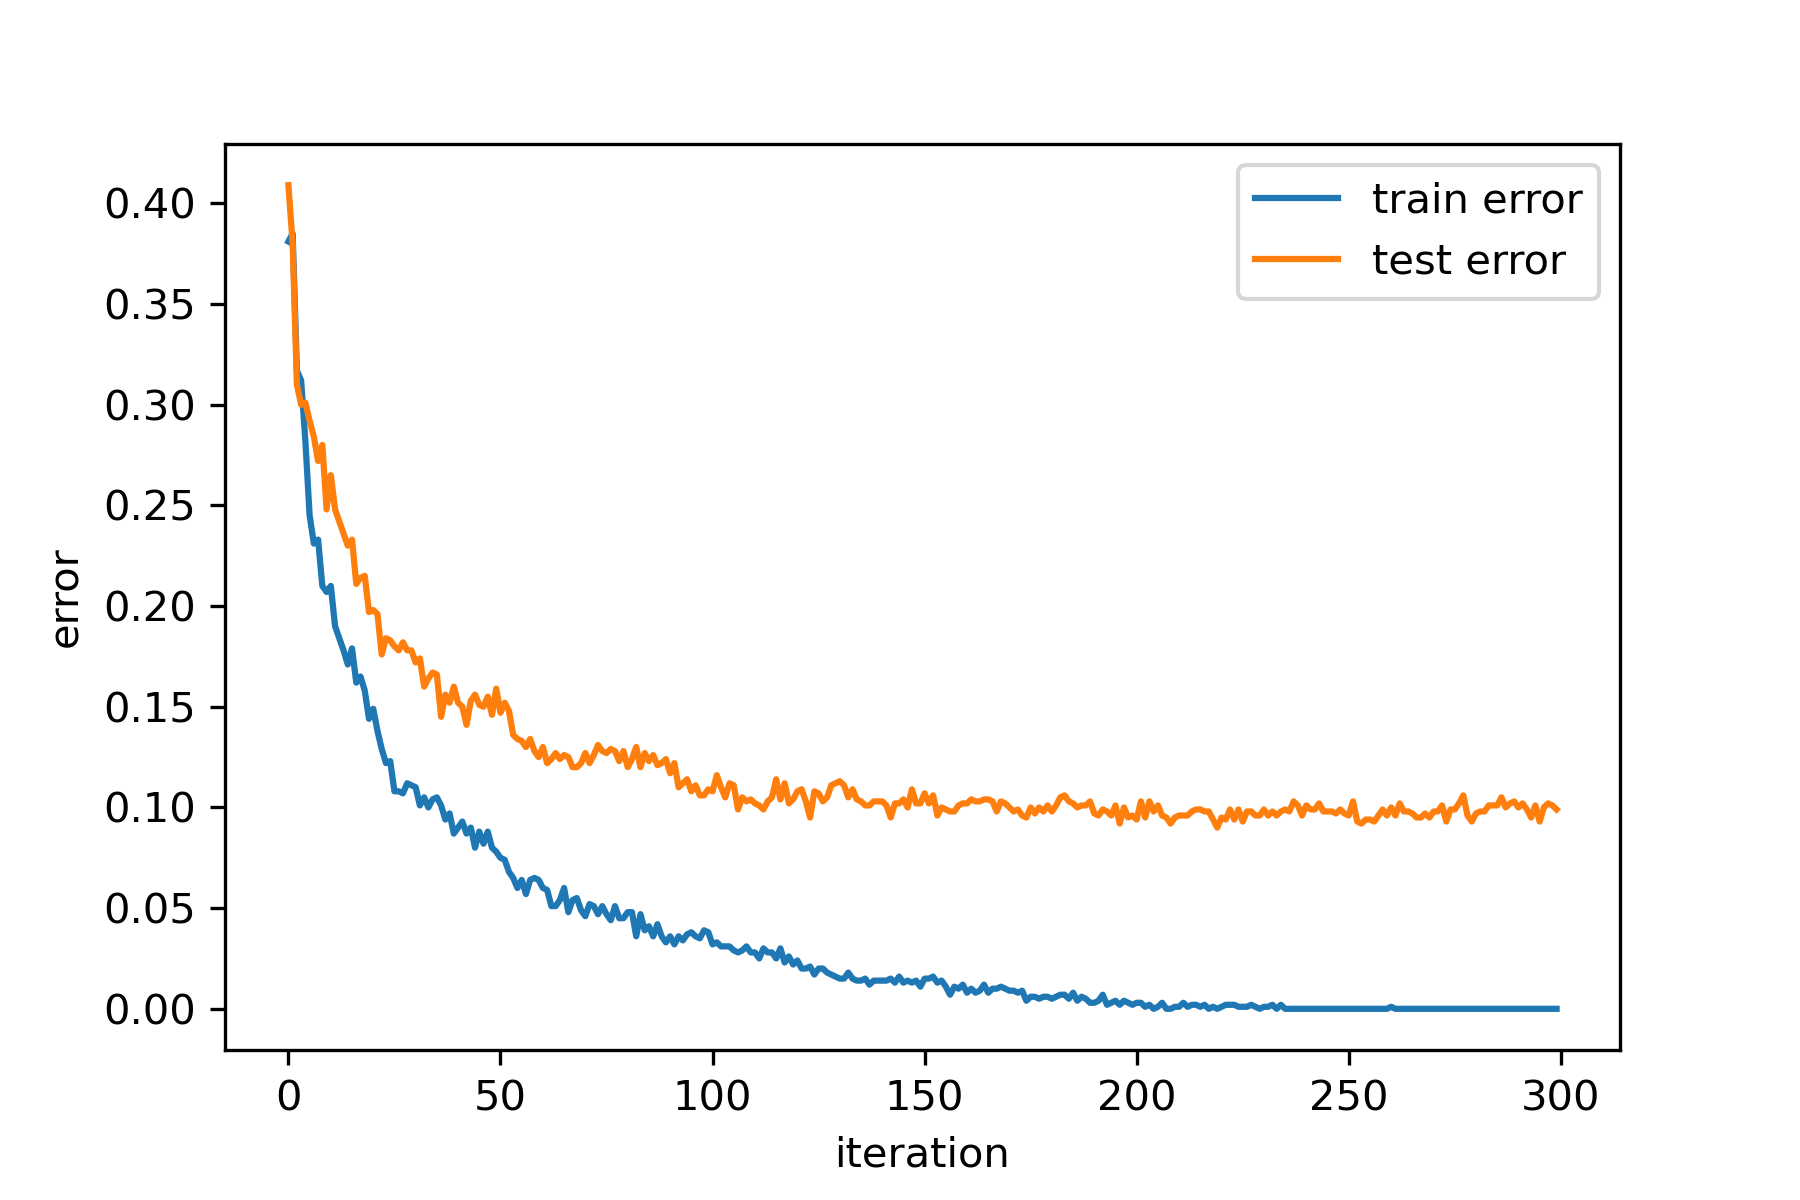
\includegraphics[width=12cm]{error.png}
  \caption{训练错误率和测试错误率}
  \label{fig:error_rate}
\end{figure}

% Reference
% \begin{thebibliography}{1}

% \bibitem{lle}

% Sam T. Roweis, lle.m - A simple matlab routine to perform LLE, Locally Linear Embedding (LLE) Code Page, \url{https://cs.nyu.edu/~roweis/lle/code.html}.

% \end{thebibliography}

\end{document}
